\documentclass{article}
\usepackage[utf8]{inputenc}
\usepackage{authblk}
\usepackage{setspace}
\usepackage[margin=1.25in]{geometry}
\usepackage{graphicx}
\usepackage{xcolor}
\usepackage{float}
\graphicspath{ {./figures/} }
\usepackage{amsmath,amssymb,amsfonts}
\usepackage{booktabs}
\usepackage{natbib}
\usepackage{hyperref}
\hypersetup{colorlinks=true, linkcolor=blue, citecolor=blue, urlcolor=blue}

\title{\textbf{Overnight versus Intraday Returns of US Mega-Cap Stocks}}
\author[1]{SIQuant Research}
\affil[1]{Hypothesis $\times$ Quant}
\date{\today}
\onehalfspacing

\begin{document}
\maketitle

\begin{abstract}
\noindent \textbf{Hypothesis:} $H_0$: the mean overnight return does not exceed the mean intraday return; $H_1$: it does \\
\textbf{Data:} 2,513 sessions of 35 US mega-caps, 2016-10-25 to 2026-10-23; 0 stock-days with a half-day move beyond 50\% dropped as data errors \\
\textbf{Method:} Open adjusted by the close adjustment factor; equal-weight daily averages; one-sided recentred stationary bootstrap of the mean difference (5,000 draws, block 10) \\
\textbf{Results:} Mean overnight 6.51 bp versus intraday 2.91 bp per day (difference 3.60 bp, $p=0.0604$); annualised 16.8\% versus 6.5\%. \\
\textbf{Research decision:} \colorbox[rgb]{0.75,0.15,0.15}{\textcolor{white}{\textbf{\,REJECTED\,}}}
\end{abstract}

\section{Design}
The decomposition follows \citet{cliff2008overnight}: the open is scaled by the dividend and split factor of the same day so that the overnight and intraday legs multiply to the adjusted close-to-close return. Equal weights across the available stocks give two daily series whose mean difference is tested.

\section{Results}
\begin{table}[H]
\centering
\caption{Mean daily overnight and intraday return of the equal-weight portfolio}
\begin{tabular}{lcc}
\toprule
Year & Overnight & Intraday \\
\midrule
2016 & 0.132\% & 0.045\% \\
2017 & 0.089\% & 0.024\% \\
2018 & 0.060\% & -0.046\% \\
2019 & 0.060\% & 0.068\% \\
2020 & 0.120\% & 0.016\% \\
2021 & 0.101\% & 0.031\% \\
2022 & -0.058\% & 0.008\% \\
2023 & 0.030\% & 0.115\% \\
2024 & 0.107\% & 0.002\% \\
2025 & 0.056\% & 0.053\% \\
2026 & 0.073\% & 0.014\% \\
\bottomrule
\end{tabular}
\end{table}


\begin{figure}[H]
\centering
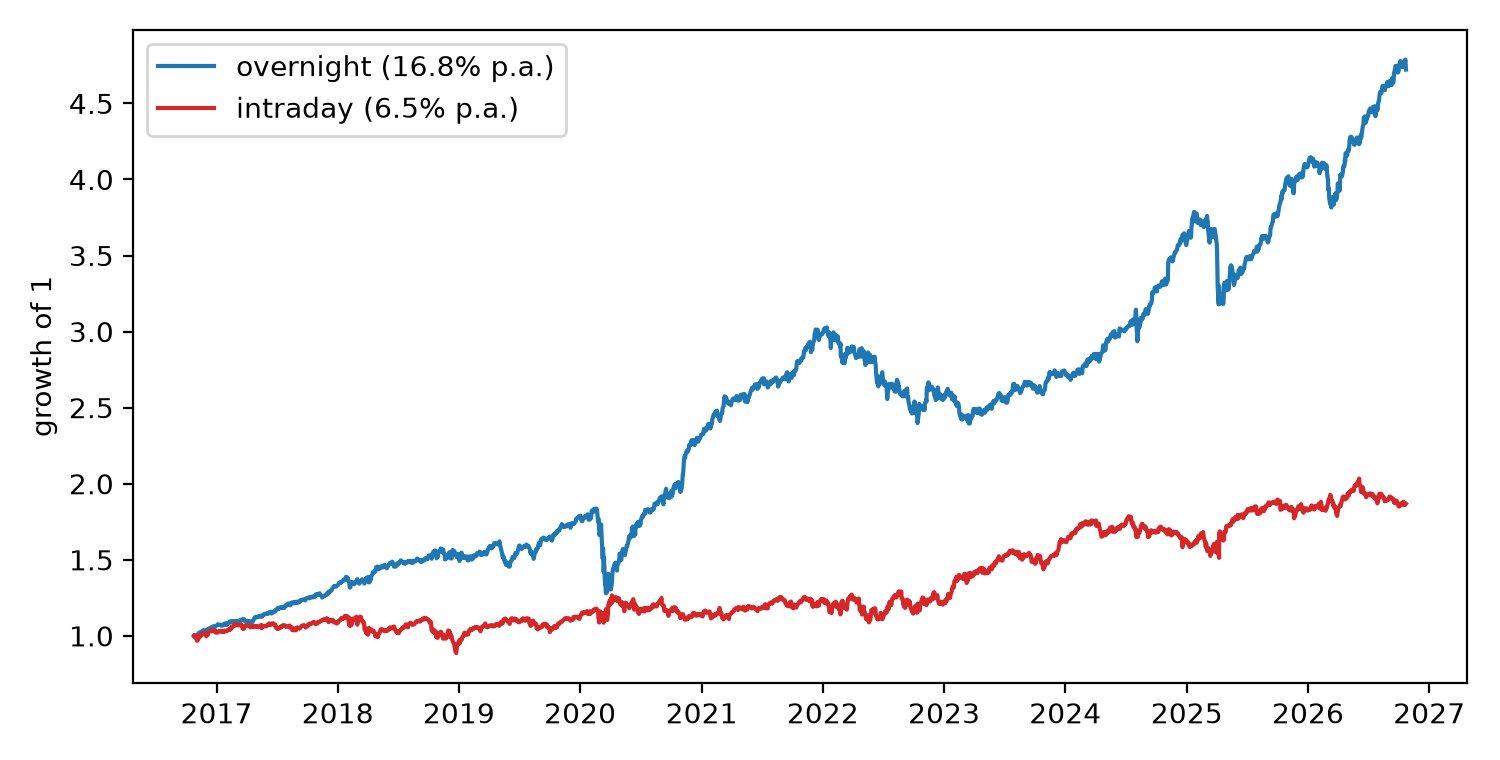
\includegraphics[width=0.8\textwidth]{fig1_overnight_vs_intraday.png}
\caption{Growth of one unit earned only overnight and only intraday.}
\end{figure}

\section{Limitations}
Opening prices on Yahoo Finance are official opening auctions; they exclude pre-market trades, so the overnight leg is the return to the opening auction, which is tradable only with market-on-open orders. The universe is today's mega-caps (survivorship) and costs are not modelled.


\bibliographystyle{plainnat}
\bibliography{references}

\end{document}
